\documentclass[xcolor={table}]{beamer}

\usetheme{Dragonfly}

\title{Introduction to Haskell\\and some category theory}
\subtitle{Wellington Functional Programming}
\projectcode{26 March 2015}
\author{Finlay Thompson}
\date{}

\AtBeginSection[]{
  \begin{frame}
  \vfill
  \centering
  \Huge
    \insertsectionhead\par%
  \vfill
  \end{frame}
}


\usepackage{fancyvrb}
\usepackage{color}



\makeatletter
\def\PY@reset{\let\PY@it=\relax \let\PY@bf=\relax%
    \let\PY@ul=\relax \let\PY@tc=\relax%
    \let\PY@bc=\relax \let\PY@ff=\relax}
\def\PY@tok#1{\csname PY@tok@#1\endcsname}
\def\PY@toks#1+{\ifx\relax#1\empty\else%
    \PY@tok{#1}\expandafter\PY@toks\fi}
\def\PY@do#1{\PY@bc{\PY@tc{\PY@ul{%
    \PY@it{\PY@bf{\PY@ff{#1}}}}}}}
\def\PY#1#2{\PY@reset\PY@toks#1+\relax+\PY@do{#2}}

\expandafter\def\csname PY@tok@gd\endcsname{\def\PY@tc##1{\textcolor[rgb]{0.63,0.00,0.00}{##1}}}
\expandafter\def\csname PY@tok@gu\endcsname{\let\PY@bf=\textbf\def\PY@tc##1{\textcolor[rgb]{0.50,0.00,0.50}{##1}}}
\expandafter\def\csname PY@tok@gt\endcsname{\def\PY@tc##1{\textcolor[rgb]{0.00,0.27,0.87}{##1}}}
\expandafter\def\csname PY@tok@gs\endcsname{\let\PY@bf=\textbf}
\expandafter\def\csname PY@tok@gr\endcsname{\def\PY@tc##1{\textcolor[rgb]{1.00,0.00,0.00}{##1}}}
\expandafter\def\csname PY@tok@cm\endcsname{\let\PY@it=\textit\def\PY@tc##1{\textcolor[rgb]{0.25,0.50,0.50}{##1}}}
\expandafter\def\csname PY@tok@vg\endcsname{\def\PY@tc##1{\textcolor[rgb]{0.10,0.09,0.49}{##1}}}
\expandafter\def\csname PY@tok@m\endcsname{\def\PY@tc##1{\textcolor[rgb]{0.40,0.40,0.40}{##1}}}
\expandafter\def\csname PY@tok@mh\endcsname{\def\PY@tc##1{\textcolor[rgb]{0.40,0.40,0.40}{##1}}}
\expandafter\def\csname PY@tok@go\endcsname{\def\PY@tc##1{\textcolor[rgb]{0.53,0.53,0.53}{##1}}}
\expandafter\def\csname PY@tok@ge\endcsname{\let\PY@it=\textit}
\expandafter\def\csname PY@tok@vc\endcsname{\def\PY@tc##1{\textcolor[rgb]{0.10,0.09,0.49}{##1}}}
\expandafter\def\csname PY@tok@il\endcsname{\def\PY@tc##1{\textcolor[rgb]{0.40,0.40,0.40}{##1}}}
\expandafter\def\csname PY@tok@cs\endcsname{\let\PY@it=\textit\def\PY@tc##1{\textcolor[rgb]{0.25,0.50,0.50}{##1}}}
\expandafter\def\csname PY@tok@cp\endcsname{\def\PY@tc##1{\textcolor[rgb]{0.74,0.48,0.00}{##1}}}
\expandafter\def\csname PY@tok@gi\endcsname{\def\PY@tc##1{\textcolor[rgb]{0.00,0.63,0.00}{##1}}}
\expandafter\def\csname PY@tok@gh\endcsname{\let\PY@bf=\textbf\def\PY@tc##1{\textcolor[rgb]{0.00,0.00,0.50}{##1}}}
\expandafter\def\csname PY@tok@ni\endcsname{\let\PY@bf=\textbf\def\PY@tc##1{\textcolor[rgb]{0.60,0.60,0.60}{##1}}}
\expandafter\def\csname PY@tok@nl\endcsname{\def\PY@tc##1{\textcolor[rgb]{0.63,0.63,0.00}{##1}}}
\expandafter\def\csname PY@tok@nn\endcsname{\let\PY@bf=\textbf\def\PY@tc##1{\textcolor[rgb]{0.00,0.00,1.00}{##1}}}
\expandafter\def\csname PY@tok@no\endcsname{\def\PY@tc##1{\textcolor[rgb]{0.53,0.00,0.00}{##1}}}
\expandafter\def\csname PY@tok@na\endcsname{\def\PY@tc##1{\textcolor[rgb]{0.49,0.56,0.16}{##1}}}
\expandafter\def\csname PY@tok@nb\endcsname{\def\PY@tc##1{\textcolor[rgb]{0.00,0.50,0.00}{##1}}}
\expandafter\def\csname PY@tok@nc\endcsname{\let\PY@bf=\textbf\def\PY@tc##1{\textcolor[rgb]{0.00,0.00,1.00}{##1}}}
\expandafter\def\csname PY@tok@nd\endcsname{\def\PY@tc##1{\textcolor[rgb]{0.67,0.13,1.00}{##1}}}
\expandafter\def\csname PY@tok@ne\endcsname{\let\PY@bf=\textbf\def\PY@tc##1{\textcolor[rgb]{0.82,0.25,0.23}{##1}}}
\expandafter\def\csname PY@tok@nf\endcsname{\def\PY@tc##1{\textcolor[rgb]{0.00,0.00,1.00}{##1}}}
\expandafter\def\csname PY@tok@si\endcsname{\let\PY@bf=\textbf\def\PY@tc##1{\textcolor[rgb]{0.73,0.40,0.53}{##1}}}
\expandafter\def\csname PY@tok@s2\endcsname{\def\PY@tc##1{\textcolor[rgb]{0.73,0.13,0.13}{##1}}}
\expandafter\def\csname PY@tok@vi\endcsname{\def\PY@tc##1{\textcolor[rgb]{0.10,0.09,0.49}{##1}}}
\expandafter\def\csname PY@tok@nt\endcsname{\let\PY@bf=\textbf\def\PY@tc##1{\textcolor[rgb]{0.00,0.50,0.00}{##1}}}
\expandafter\def\csname PY@tok@nv\endcsname{\def\PY@tc##1{\textcolor[rgb]{0.10,0.09,0.49}{##1}}}
\expandafter\def\csname PY@tok@s1\endcsname{\def\PY@tc##1{\textcolor[rgb]{0.73,0.13,0.13}{##1}}}
\expandafter\def\csname PY@tok@sh\endcsname{\def\PY@tc##1{\textcolor[rgb]{0.73,0.13,0.13}{##1}}}
\expandafter\def\csname PY@tok@sc\endcsname{\def\PY@tc##1{\textcolor[rgb]{0.73,0.13,0.13}{##1}}}
\expandafter\def\csname PY@tok@sx\endcsname{\def\PY@tc##1{\textcolor[rgb]{0.00,0.50,0.00}{##1}}}
\expandafter\def\csname PY@tok@bp\endcsname{\def\PY@tc##1{\textcolor[rgb]{0.00,0.50,0.00}{##1}}}
\expandafter\def\csname PY@tok@c1\endcsname{\let\PY@it=\textit\def\PY@tc##1{\textcolor[rgb]{0.25,0.50,0.50}{##1}}}
\expandafter\def\csname PY@tok@kc\endcsname{\let\PY@bf=\textbf\def\PY@tc##1{\textcolor[rgb]{0.00,0.50,0.00}{##1}}}
\expandafter\def\csname PY@tok@c\endcsname{\let\PY@it=\textit\def\PY@tc##1{\textcolor[rgb]{0.25,0.50,0.50}{##1}}}
\expandafter\def\csname PY@tok@mf\endcsname{\def\PY@tc##1{\textcolor[rgb]{0.40,0.40,0.40}{##1}}}
\expandafter\def\csname PY@tok@err\endcsname{\def\PY@bc##1{\setlength{\fboxsep}{0pt}\fcolorbox[rgb]{1.00,0.00,0.00}{1,1,1}{\strut ##1}}}
\expandafter\def\csname PY@tok@kd\endcsname{\let\PY@bf=\textbf\def\PY@tc##1{\textcolor[rgb]{0.00,0.50,0.00}{##1}}}
\expandafter\def\csname PY@tok@ss\endcsname{\def\PY@tc##1{\textcolor[rgb]{0.10,0.09,0.49}{##1}}}
\expandafter\def\csname PY@tok@sr\endcsname{\def\PY@tc##1{\textcolor[rgb]{0.73,0.40,0.53}{##1}}}
\expandafter\def\csname PY@tok@mo\endcsname{\def\PY@tc##1{\textcolor[rgb]{0.40,0.40,0.40}{##1}}}
\expandafter\def\csname PY@tok@kn\endcsname{\let\PY@bf=\textbf\def\PY@tc##1{\textcolor[rgb]{0.00,0.50,0.00}{##1}}}
\expandafter\def\csname PY@tok@mi\endcsname{\def\PY@tc##1{\textcolor[rgb]{0.40,0.40,0.40}{##1}}}
\expandafter\def\csname PY@tok@gp\endcsname{\let\PY@bf=\textbf\def\PY@tc##1{\textcolor[rgb]{0.00,0.00,0.50}{##1}}}
\expandafter\def\csname PY@tok@o\endcsname{\def\PY@tc##1{\textcolor[rgb]{0.40,0.40,0.40}{##1}}}
\expandafter\def\csname PY@tok@kr\endcsname{\let\PY@bf=\textbf\def\PY@tc##1{\textcolor[rgb]{0.00,0.50,0.00}{##1}}}
\expandafter\def\csname PY@tok@s\endcsname{\def\PY@tc##1{\textcolor[rgb]{0.73,0.13,0.13}{##1}}}
\expandafter\def\csname PY@tok@kp\endcsname{\def\PY@tc##1{\textcolor[rgb]{0.00,0.50,0.00}{##1}}}
\expandafter\def\csname PY@tok@w\endcsname{\def\PY@tc##1{\textcolor[rgb]{0.73,0.73,0.73}{##1}}}
\expandafter\def\csname PY@tok@kt\endcsname{\def\PY@tc##1{\textcolor[rgb]{0.69,0.00,0.25}{##1}}}
\expandafter\def\csname PY@tok@ow\endcsname{\let\PY@bf=\textbf\def\PY@tc##1{\textcolor[rgb]{0.67,0.13,1.00}{##1}}}
\expandafter\def\csname PY@tok@sb\endcsname{\def\PY@tc##1{\textcolor[rgb]{0.73,0.13,0.13}{##1}}}
\expandafter\def\csname PY@tok@k\endcsname{\let\PY@bf=\textbf\def\PY@tc##1{\textcolor[rgb]{0.00,0.50,0.00}{##1}}}
\expandafter\def\csname PY@tok@se\endcsname{\let\PY@bf=\textbf\def\PY@tc##1{\textcolor[rgb]{0.73,0.40,0.13}{##1}}}
\expandafter\def\csname PY@tok@sd\endcsname{\let\PY@it=\textit\def\PY@tc##1{\textcolor[rgb]{0.73,0.13,0.13}{##1}}}

\def\PYZbs{\char`\\}
\def\PYZus{\char`\_}
\def\PYZob{\char`\{}
\def\PYZcb{\char`\}}
\def\PYZca{\char`\^}
\def\PYZam{\char`\&}
\def\PYZlt{\char`\<}
\def\PYZgt{\char`\>}
\def\PYZsh{\char`\#}
\def\PYZpc{\char`\%}
\def\PYZdl{\char`\$}
\def\PYZhy{\char`\-}
\def\PYZsq{\char`\'}
\def\PYZdq{\char`\"}
\def\PYZti{\char`\~}
% for compatibility with earlier versions
\def\PYZat{@}
\def\PYZlb{[}
\def\PYZrb{]}
\makeatother



\usepackage{framed}
\renewenvironment{leftbar}[1][\hsize]
{% 
\def\FrameCommand 
{%

    {\color{lightgray}\vrule width 3pt}%
    \hspace{0pt}%must no space.
    \fboxsep=\FrameSep\colorbox{white}%
}%
\MakeFramed{\hsize#1\advance\hsize-\width\FrameRestore}%
}
{\endMakeFramed}

\begin{document}

\titleslide

\section{Introduction}

\begin{frame}{}{}

    \begin{columns}
    \column{0.5\textwidth}
    {\Large Haskell is strange ? }

    \pause\bigskip
    Strongly typed functional programming language

    \pause\bigskip
    Lazy evaluation
    
    \pause\bigskip
    Pure functions with no side effects 
    
    \pause\bigskip
    Fairly old\pause, fairly odd

    \column{0.5\textwidth}
    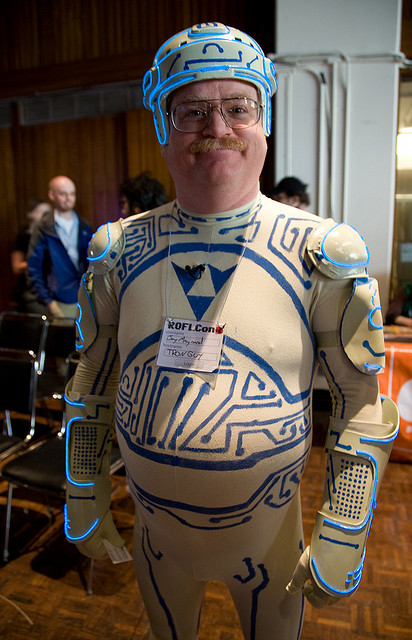
\includegraphics[width=0.9\textwidth]{images/tron-guy.jpg}
        
    \end{columns}

\end{frame}

\begin{frame}{}{}

    \begin{columns}
    \column{0.5\textwidth}
    {\Large Haskell is hard ?}

    \pause\bigskip
    My program won't compile,\\ and I don't know why ?

    \pause\bigskip
    The tutorials online are confusing.

    \pause\bigskip
    Oh god, I am reading math !

    \pause\bigskip
    Huh ?

    \column{0.5\textwidth}
    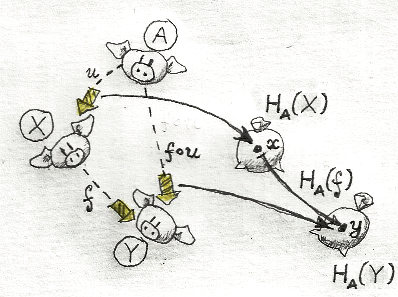
\includegraphics[width=0.9\textwidth]{images/content-proxy.png}
        
    \end{columns}

\end{frame}

\begin{frame}{}{}

    \begin{columns}
    \column{0.5\textwidth}
    {\Large Haskell is impractical ? }

    \pause\bigskip
    Strong type system gets in the way

    \pause\bigskip
    Hard to install compiler, and find good libraries

    \pause\bigskip
    Compiled code is slow

    \pause\bigskip
    Impossible to find developers

    \pause

    \column{0.5\textwidth}
    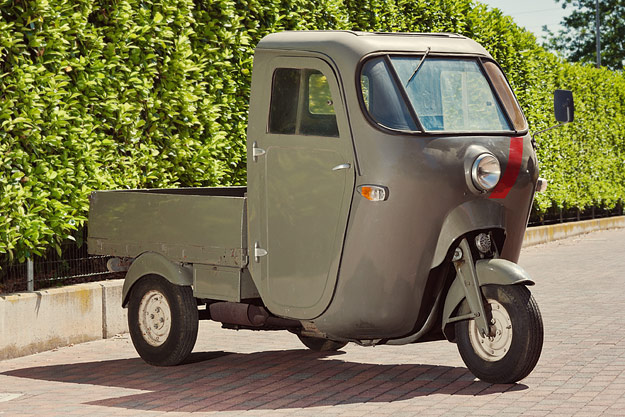
\includegraphics[width=0.9\textwidth]{images/ducati-muletto.jpg}
        
    \end{columns}

\end{frame}

\begin{frame}{}{}

    {\Large Haskell is awesome! }

    \pause
    Is Haskell weird ?\pause
    \begin{itemize}
        \item No, just different. All other languages are weird.
    \end{itemize}

    \pause
    Is Haskell hard ?\pause 
    \begin{itemize}
        \item No, but it makes you think differently, which is good.
    \end{itemize}

    \pause
    Is Haskell impractical ?\pause 
    \begin{itemize}
        \item Hackage has thousands of libraries
        \item Haskell is very fast, and getting faster
        \item Community is growing quickly
    \end{itemize}

\end{frame}

\begin{frame}{}{}

    \centering
    {\Large To learn Haskell, \par it helps to learn a little category theory. }
    \par\bigskip\pause

    Actually, I reckon you already know category theory!


\end{frame}

\section{Anatomy of a function}

\begin{frame}{}{}

    \centering
    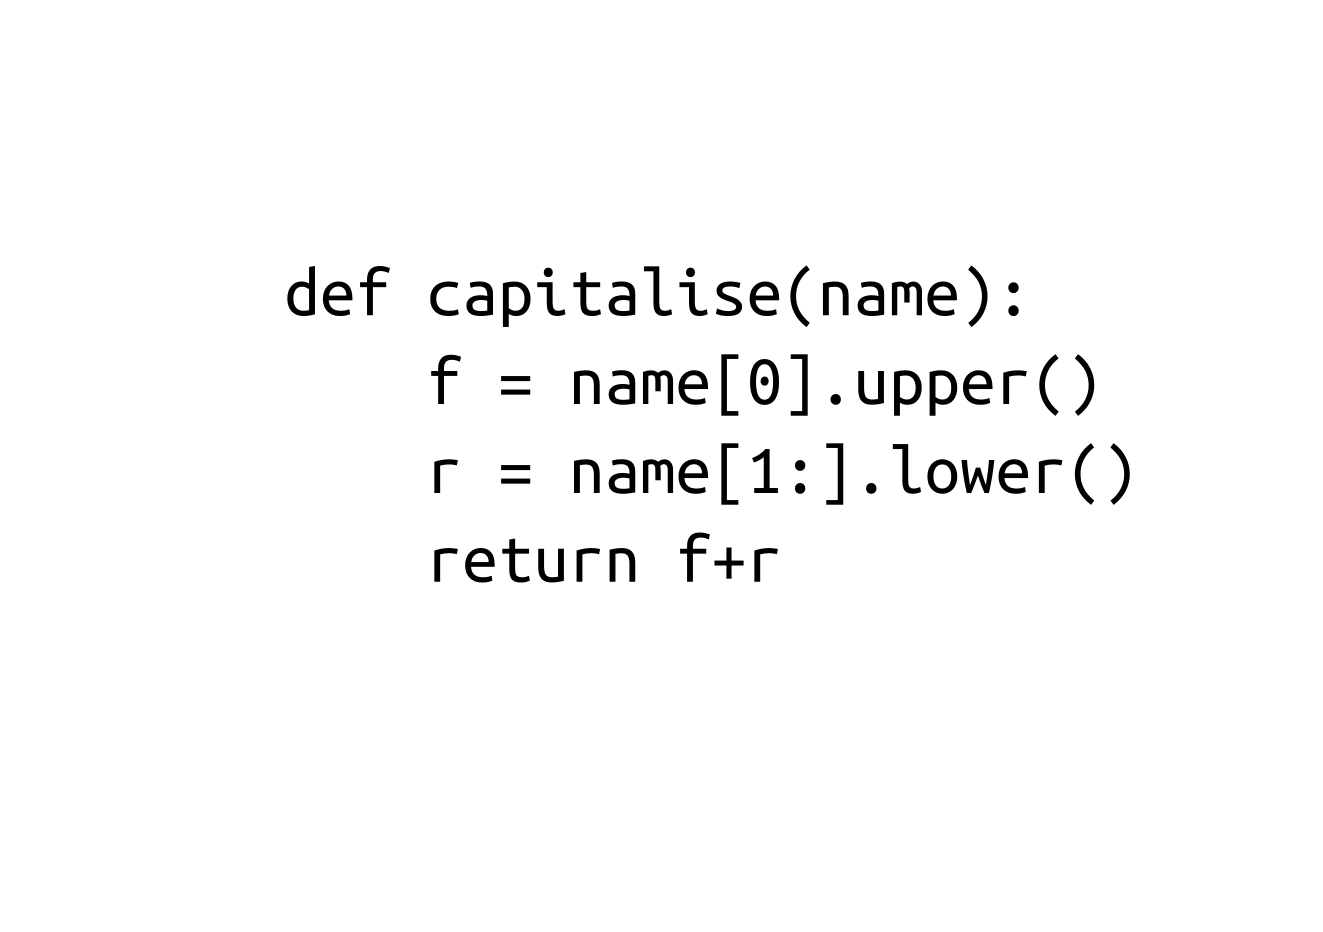
\includegraphics[width=0.9\textwidth]{images/python-code-01.png}

\end{frame}

\begin{frame}{}{}

    \centering
    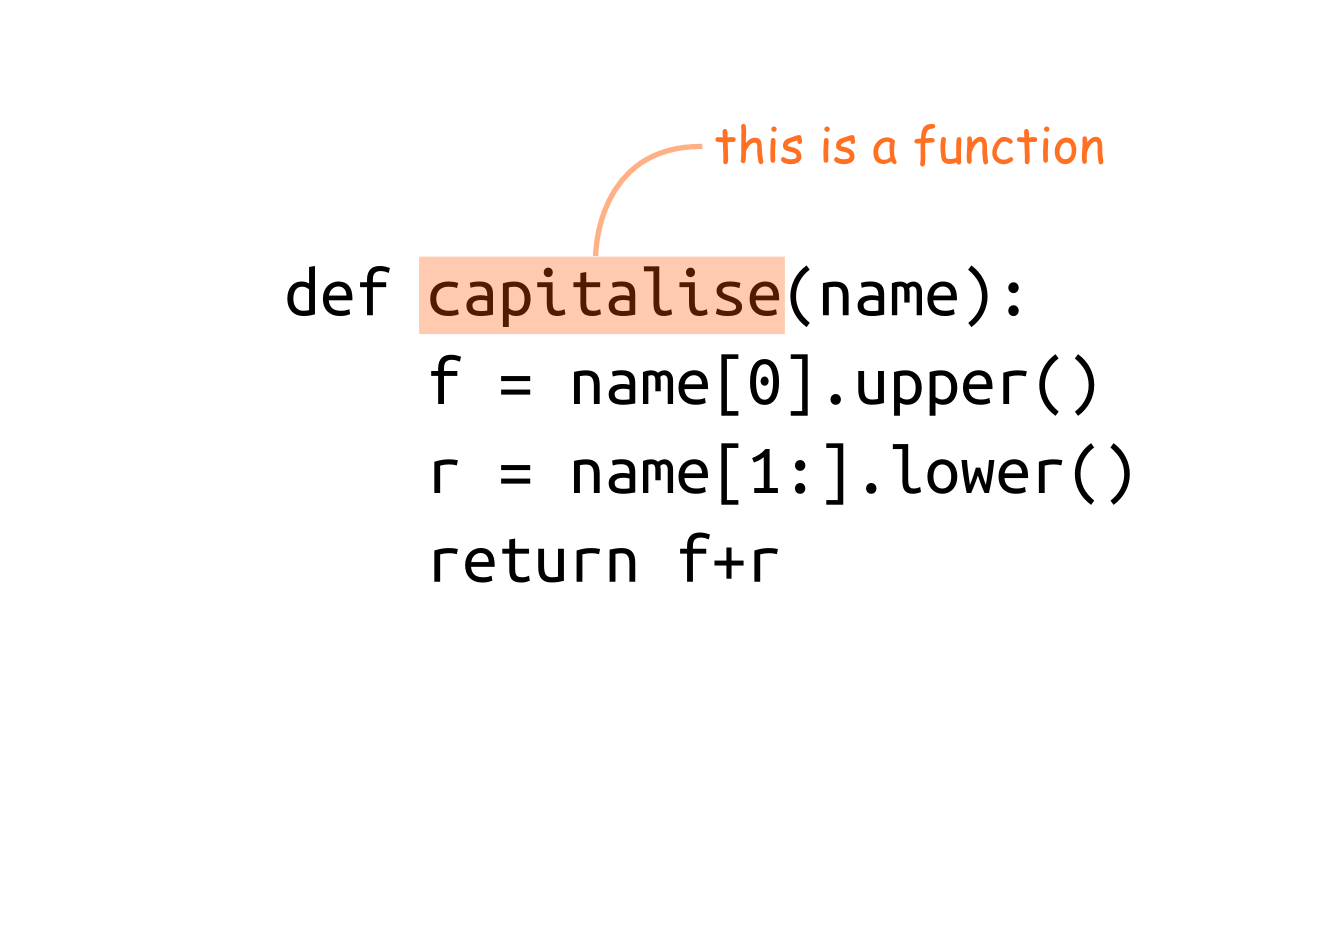
\includegraphics[width=0.9\textwidth]{images/python-code-02.png}

\end{frame}

\begin{frame}{}{}

    \centering
    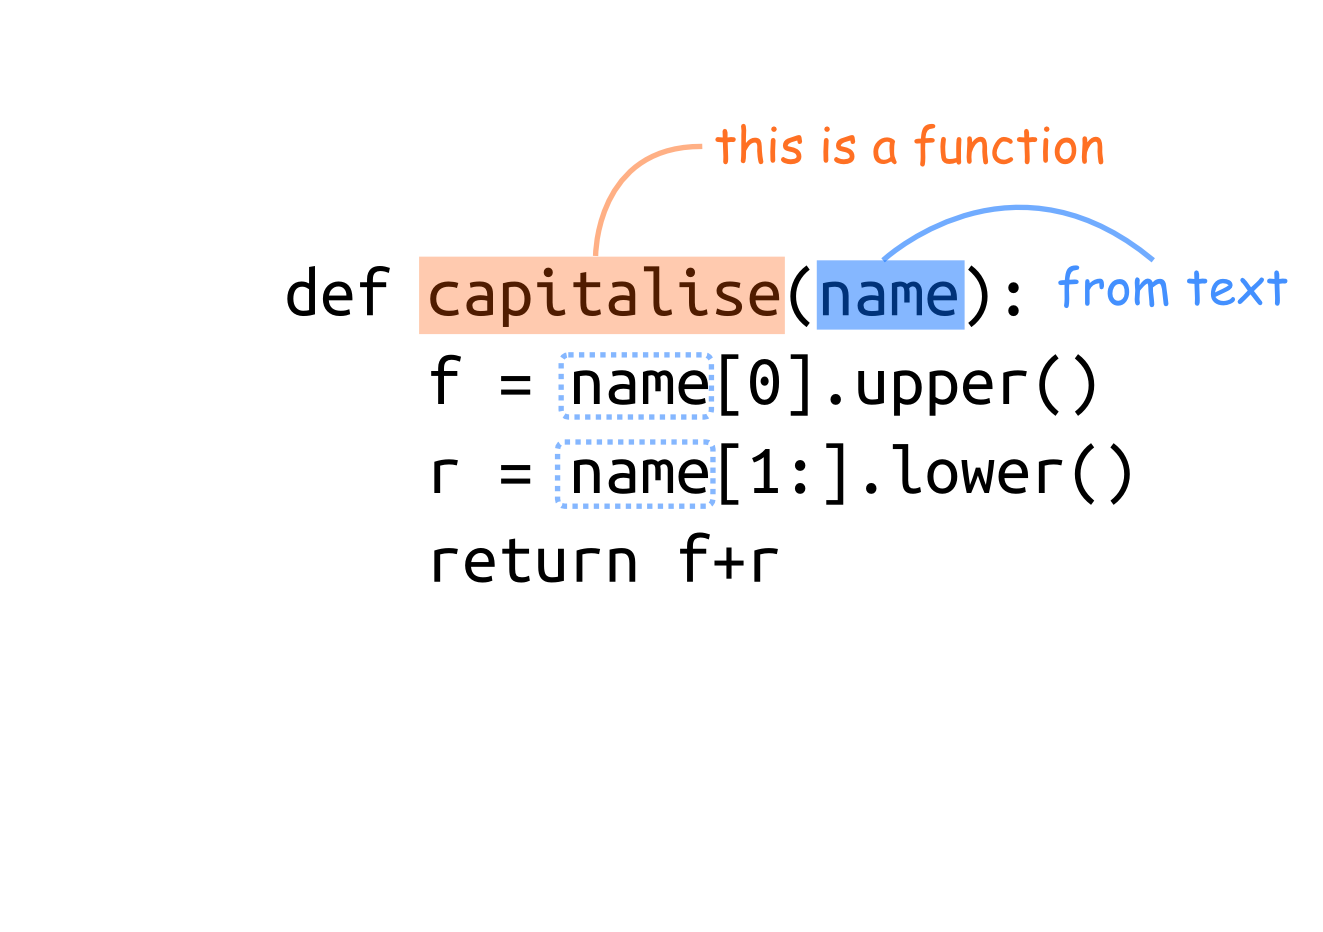
\includegraphics[width=0.9\textwidth]{images/python-code-03.png}

\end{frame}

\begin{frame}{}{}

    \centering
    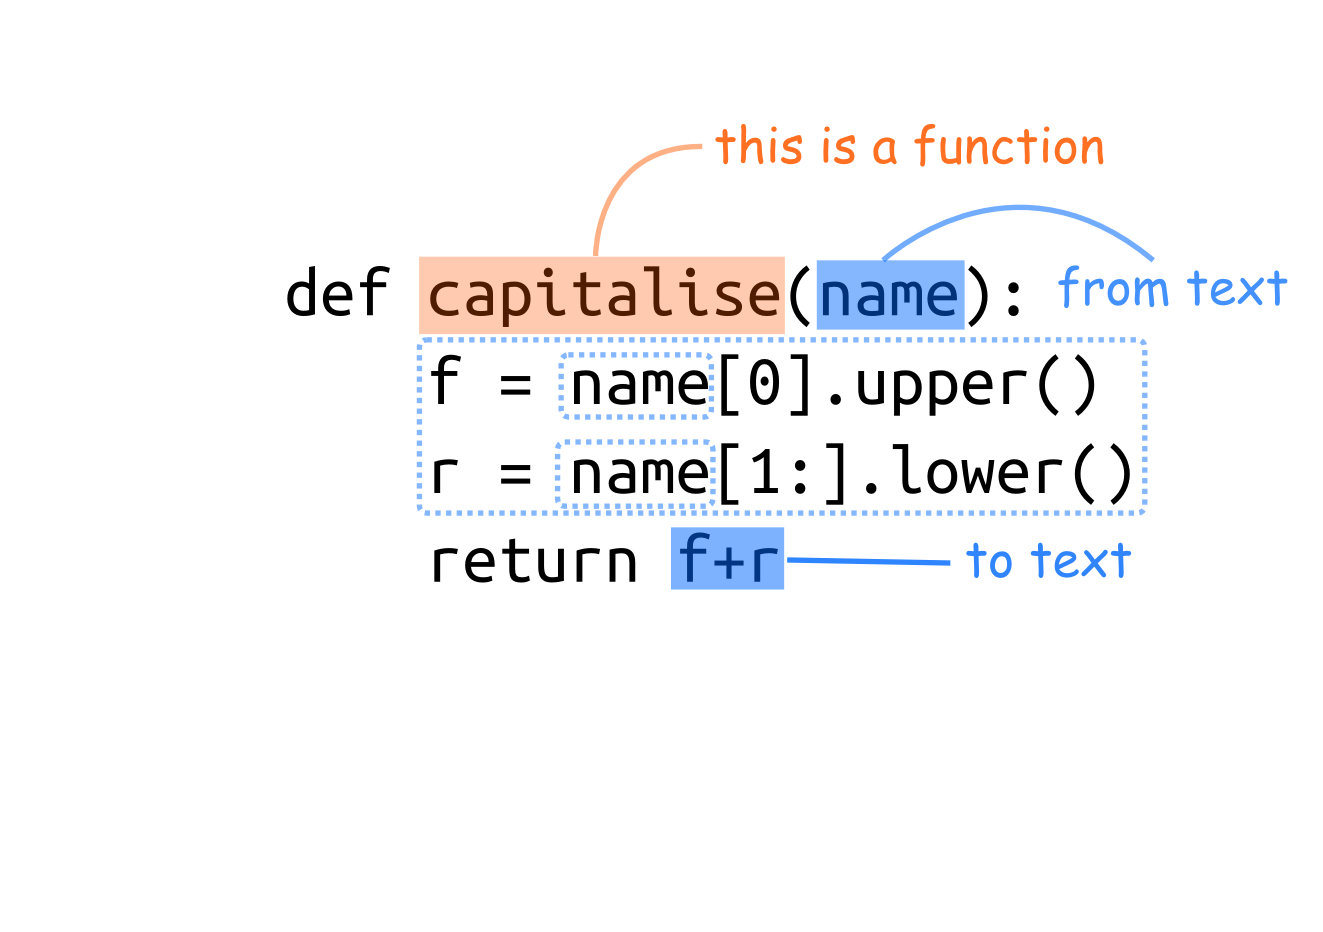
\includegraphics[width=0.9\textwidth]{images/python-code-04.png}

\end{frame}

\begin{frame}{}{}

    \centering
    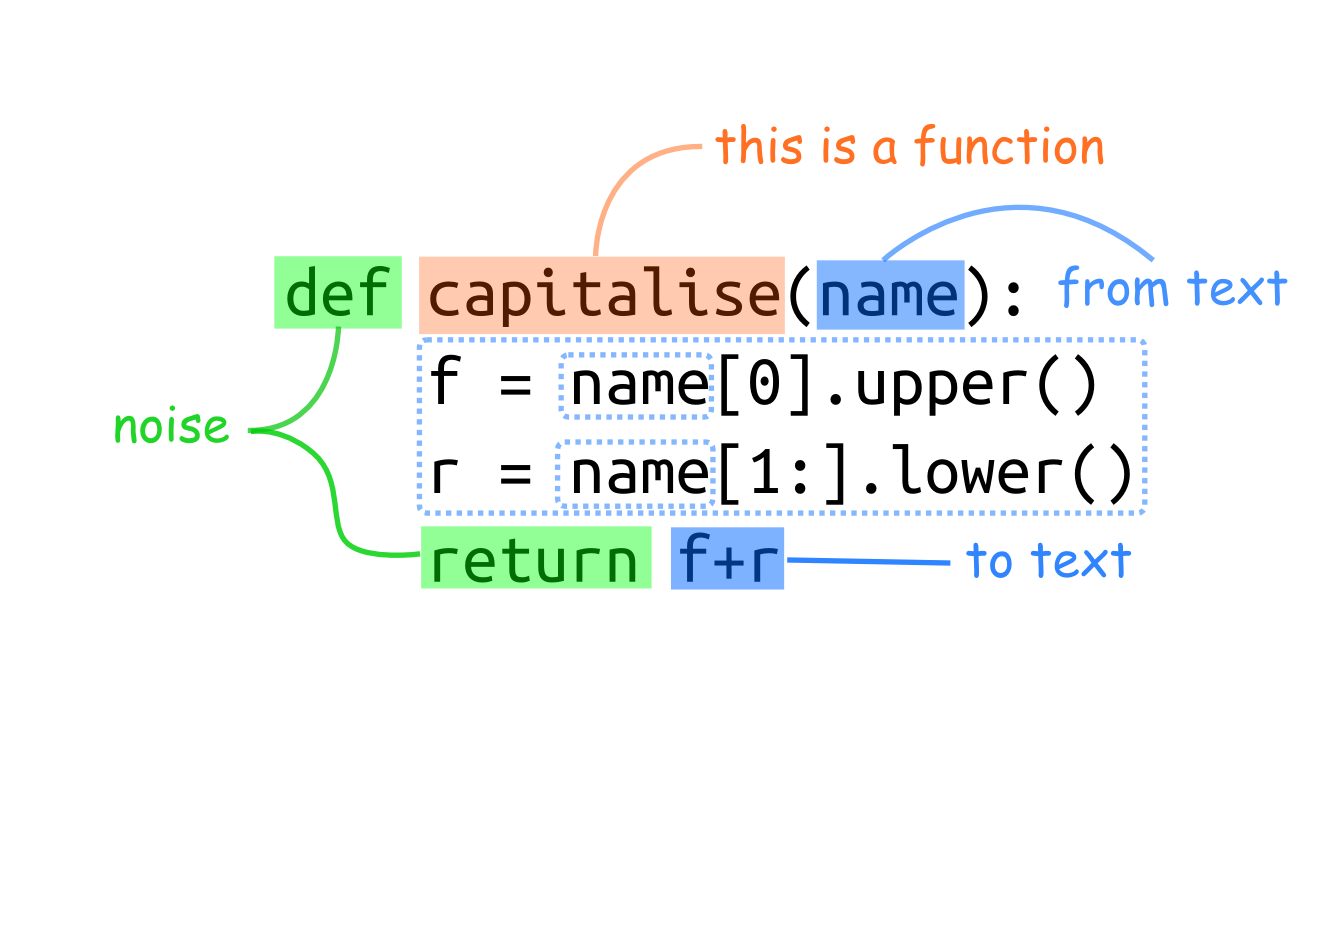
\includegraphics[width=0.9\textwidth]{images/python-code-05.png}

\end{frame}


\begin{frame}{}{}

    \centering
    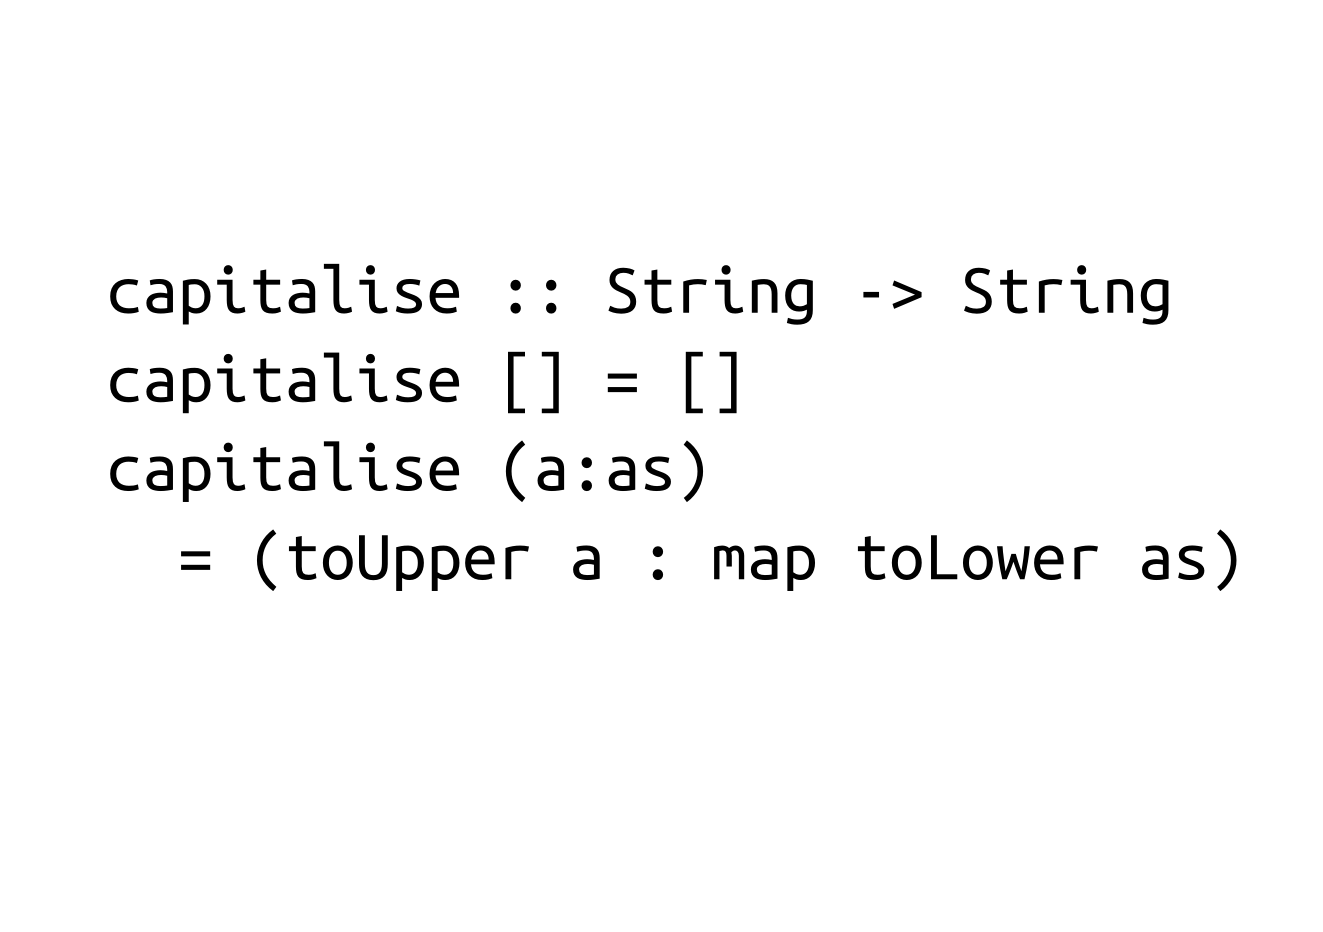
\includegraphics[width=0.9\textwidth]{images/haskell-code-01.png}

\end{frame}

\begin{frame}{}{}

    \centering
    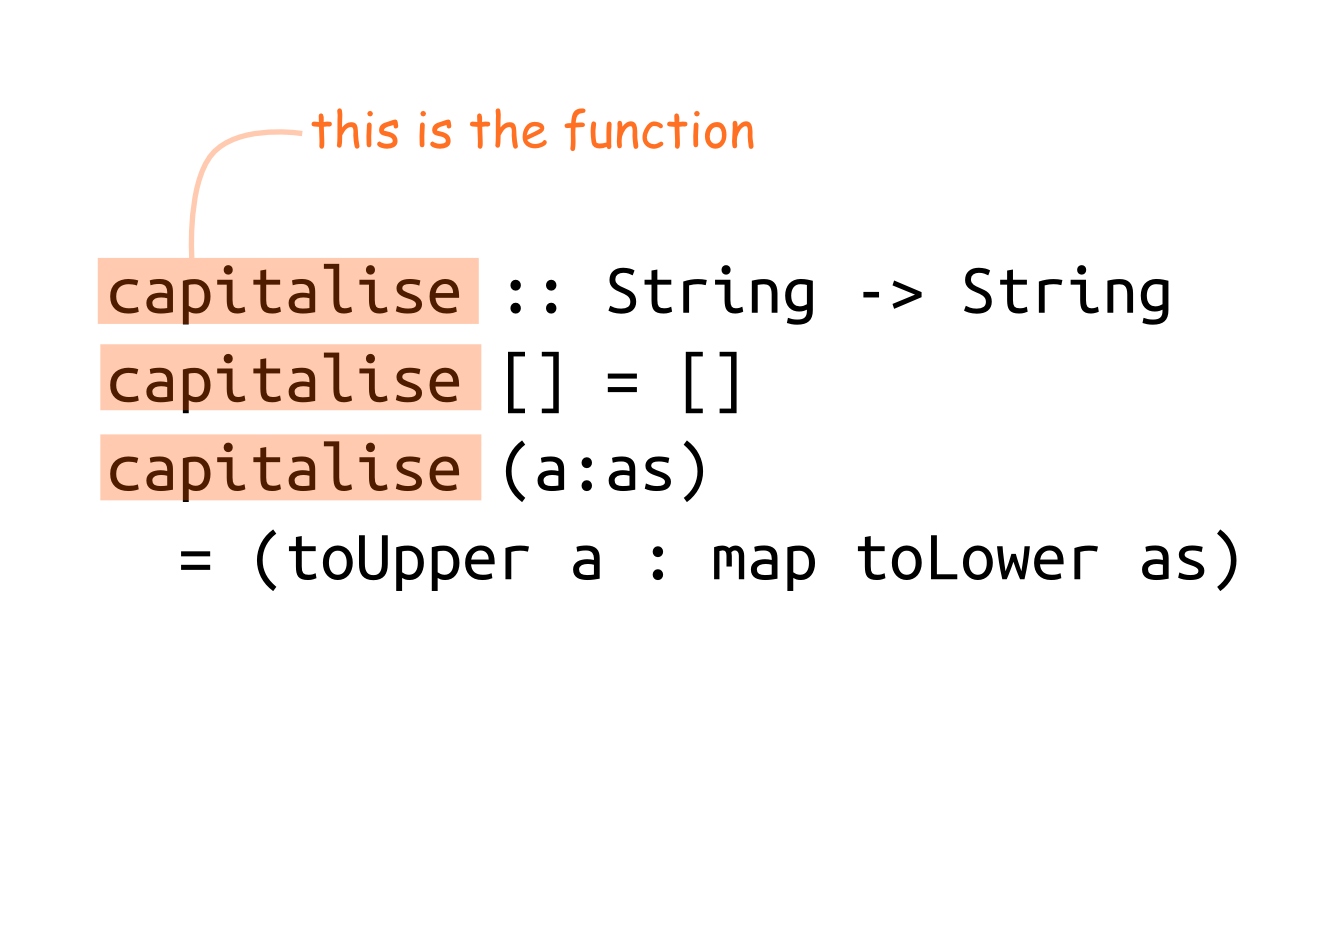
\includegraphics[width=0.9\textwidth]{images/haskell-code-02.png}

\end{frame}

\begin{frame}{}{}

    \centering
    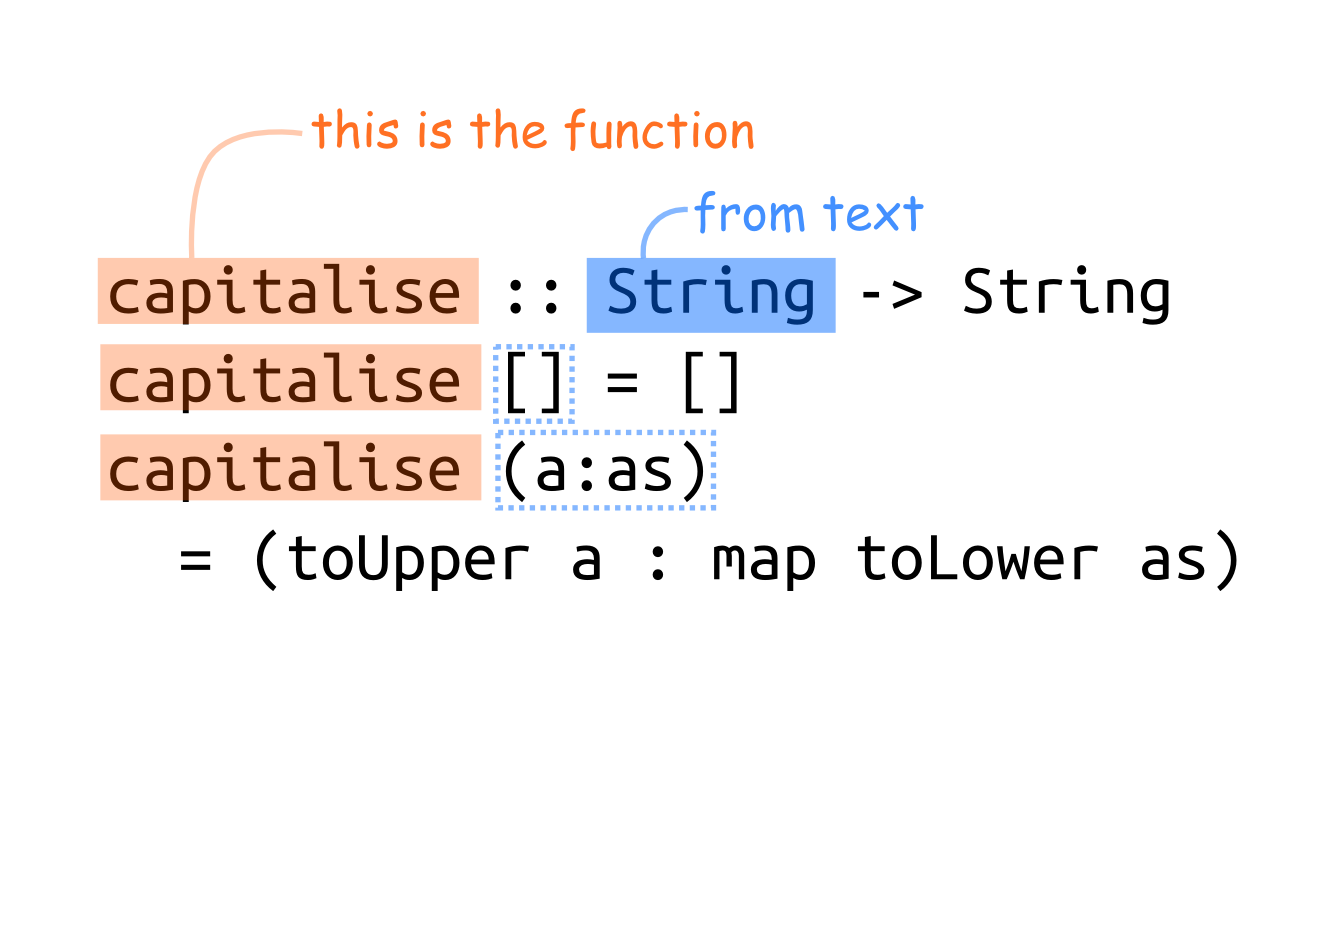
\includegraphics[width=0.9\textwidth]{images/haskell-code-03.png}

\end{frame}

\begin{frame}{}{}

    \centering
    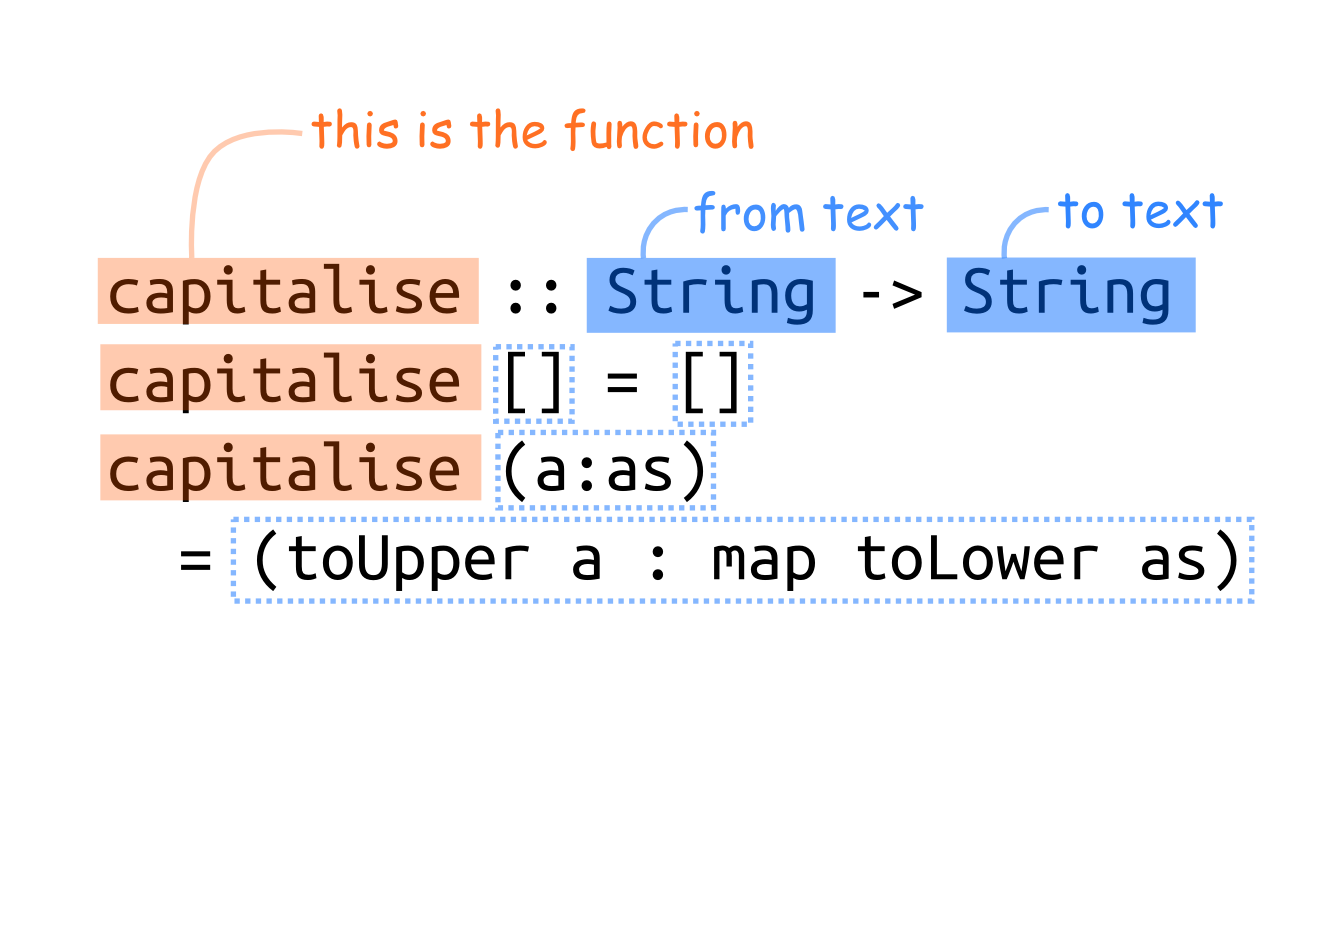
\includegraphics[width=0.9\textwidth]{images/haskell-code-04.png}

\end{frame}

\begin{frame}{}{}

    \centering
    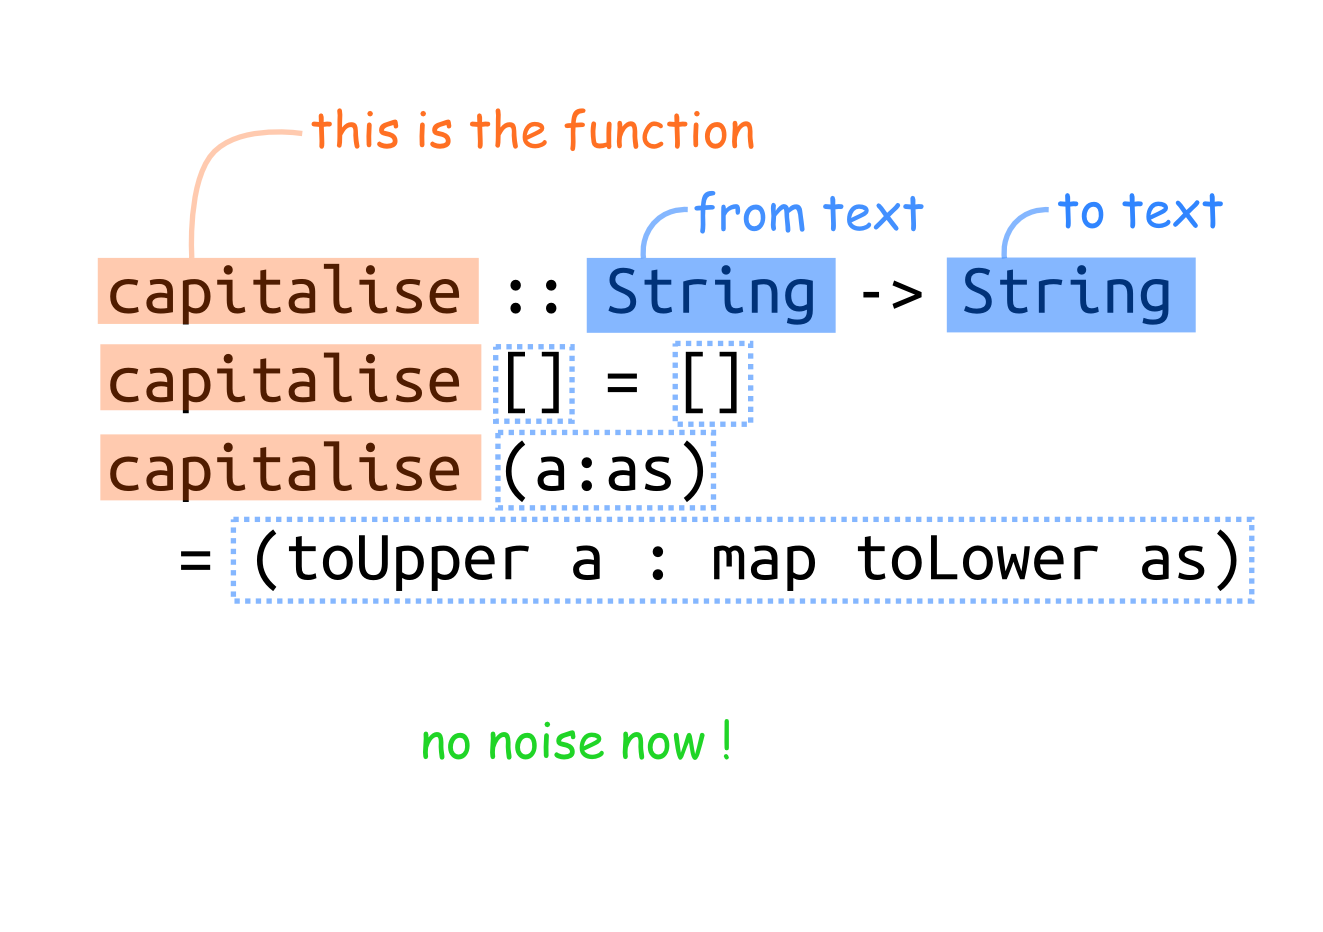
\includegraphics[width=0.9\textwidth]{images/haskell-code-05.png}

\end{frame}


\section{A little category theory}

\begin{frame}{}{}

    \centering
    \only<1>{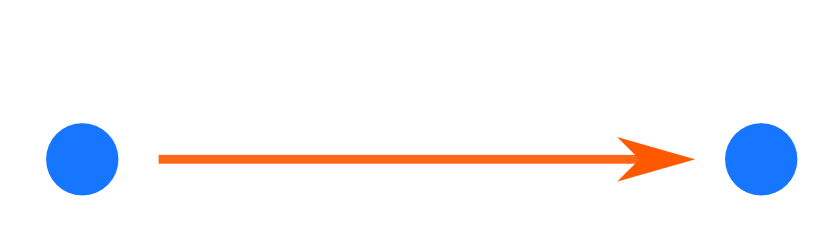
\includegraphics[width=0.7\textwidth]{images/two-dots-01.png}}

    \only<2>{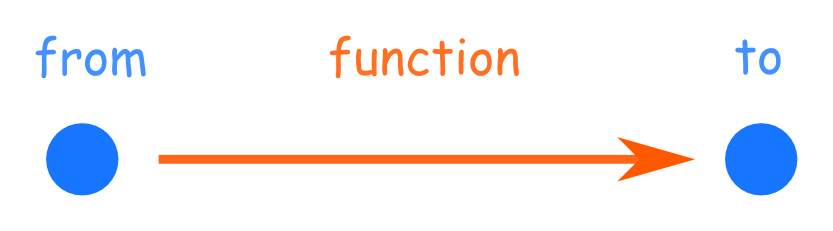
\includegraphics[width=0.7\textwidth]{images/two-dots-02.png}}

\end{frame}

\begin{frame}{}{}

    {\Large Category theory is all about arrows. }

    \pause\bigskip
    Need to define what the \textbf{objects} are.

    \pause\bigskip
    Between two objects, there are \textbf{arrows}. 

    \pause\bigskip
    There are some rules, more on that later.

\end{frame}

\begin{frame}{}{}

    {\Large Programming involves defining arrows.}

    \pause\bigskip
    The objects in the programming category are \textbf{types}. Types are sets of values.

    \pause\bigskip
    Writing functions in a programming language involves defining arrows between data types. 

    \pause\bigskip
    Haskell emphasises category theory aspect of programming.

\end{frame}

\begin{frame}{}{}

    \emph{Warning, philosophical musing ahead...}

    \pause\bigskip
    Category theory is \textbf{about} the common patterns that emerge when we consider diagrams of objects and arrows.

    \pause\bigskip
    A category defines some kind of objects, and the way we can transform these objects into each other. It is a very general concept, and so almost completely vacuous.

    \pause\bigskip
    As is often the case with mathematical concepts, there is nothing more than the definitions.

\end{frame}

\begin{frame}{}{}

    \begin{columns}
    \column{0.75\textwidth}
    
    \begin{definition}
        A category $C$ consists of
        \begin{itemize}
            \item a class of objects $Obj(C)$, 
            \item $\forall X,Y\in Obj(C)$, $\exists\ $ a class of arrows $C(X,Y)$.
            \item $\forall f:X\to Y$, and $g:Y \to Z$, $\exists\ g\circ f:X \to Z$.
        \end{itemize}
        Such that
        \begin{itemize}
            \item $\forall X\in Obj(C)$, $\exists\ id_X: X \to X$,
            \item $\forall f:X\to Y$, then 
                $$ f \circ id_X = f = id_Y \circ f $$
            \item $\forall f:X\to Y$, $g:Y \to Z$, and $h:Z \to W$, then
                $$ (h \circ g) \circ f = h \circ (g \circ f) $$
        \end{itemize}
    \end{definition}


    \column{0.25\textwidth}
    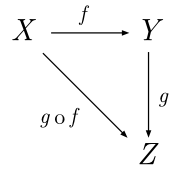
\includegraphics[width=\textwidth]{images/Commutative_diagram_for_morphism.png}
    \end{columns}

\end{frame}

\section{Programming in patterns}

\begin{frame}{}{}

    {\Large The history of computer programming has involved the discovering patterns.}

    \pause\bigskip
    Subroutines emerged as a pattern from assembly and fortran, and became the central concept in C. 

    \pause\bigskip
    Associating functions with structs emerged as a pattern in C, and became object classes in C++.  

    \pause\bigskip
    Numerous patterns have emerged from mainstream object-oriented languages such as Java, C\#, and C++.

\end{frame}

\begin{frame}{}{}

    {\Large Category theory provides Haskell with patterns.}

    \pause\bigskip
    The Haskell language has it's origins in the lambda calculus, and is strongly influenced by ideas category theory.

    \pause\bigskip
    The Haskell community draws on category theory to provide programming patterns.

    \pause\bigskip
    They \emph{tend} to be good patterns, with good performance characteristics, and general enough to be useful.

\end{frame}

\section{Pattern: Functors}

\begin{frame}{}{}

    {\Large Functors are arrows between categories.}

    \pause\bigskip
    \begin{definition}
        A Functor $F : C \to D$ consists of
        \begin{itemize}
            \item A map $F: Obj(C) \to Obj(D)$,
            \item $\forall\ X,Y\in Obj(C)$, a map $F: C(X,Y) \to D(FX, FY)$
        \end{itemize}
        Such that
        \begin{itemize}
            \item $\forall\ X\in C$, then $ F(id_X) = id_{FX} $
            \item $\forall\ f:X\to Y, g:Y\to Z$, then $ F(g \circ f) = F(g) \circ F(f) $
        \end{itemize}
    \end{definition}

\end{frame}

\begin{frame}[fragile]{}{}

    {\Large User defined data types in Haskell }

    \pause\bigskip
    The \textbf{data} keyword creates new data types in Haskell. 
    
    \pause\bigskip
    They can take other types as parameters, creating mappings from Haskell types to Haskell types, the beginning of a Functor.

    \pause\bigskip
    For example, the maybe type allows for ``nullable'' types.
    \begin{leftbar}
    \input{maybe.pyg}
    \end{leftbar}

\end{frame}

\begin{frame}[fragile]{}{}

    {\Large Functors modify the arrows too.}

    \pause\bigskip
    \begin{leftbar}
        \input{functor-class.pyg}
    \end{leftbar}

    \pause\bigskip
    \begin{leftbar}
        \input{functor-instance.pyg}
    \end{leftbar}

\end{frame}

\begin{frame}[fragile]{}{}

    \begin{leftbar}
        \input{functor-example.pyg}
    \end{leftbar}

\end{frame}

\begin{frame}[fragile]{}{}

    {\Large The Functor pattern successfully separates concerns}

    \pause\bigskip
    Define a function that does something in your domain.

    \pause\bigskip
    Separately, define a Functor instance for a wrapper data type.

    \pause\bigskip
    Use the wrapped values as if they were not wrapped!

\end{frame}



\begin{frame}{}{}

{\Large Further reading}

The official Haskell website is good \\
\url{https://www.haskell.org/}
\bigskip

Newish book all about the Maybe data type\\
\url{https://gumroad.com/l/maybe-haskell/}
\bigskip

Good series of blog posts on category theory\\
\url{ http://bartoszmilewski.com/2014/10/28/category-theory-for-programmers-the-preface/}

\end{frame}



\end{document}
